% Class pixel frequency on the RUGD TRAINING split (non-void pixels), log scale.
% Data: results/class_freq_rugd.csv (scripts/compute_class_weights.py).
% bridge (0 training pixels) cannot be drawn on a log axis and is noted in the caption.
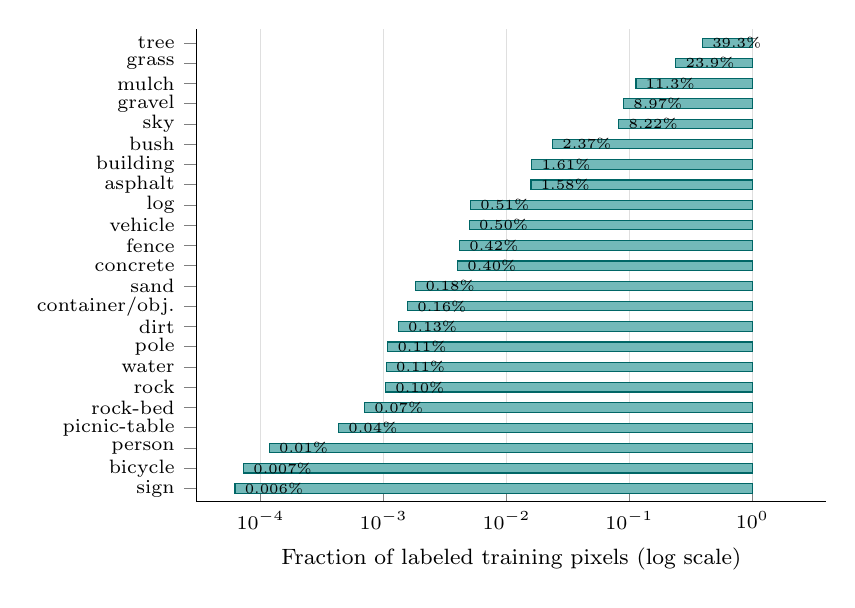
\begin{tikzpicture}
\begin{axis}[
  xbar,
  scale only axis,
  width=0.66\linewidth,
  height=6.0cm,
  bar width=3.4pt,
  xmode=log,
  log basis x=10,
  xmin=3e-5, xmax=4,
  xtick={1e-4,1e-3,1e-2,1e-1,1},
  xlabel={Fraction of labeled training pixels (log scale)},
  xlabel style={font=\footnotesize},
  symbolic y coords={sign,bicycle,person,picnic-table,rock-bed,rock,water,pole,dirt,container/obj.,sand,concrete,fence,vehicle,log,asphalt,building,bush,sky,gravel,mulch,grass,tree},
  ytick=data,
  y tick label style={font=\scriptsize},
  x tick label style={font=\scriptsize},
  enlarge y limits=0.03,
  axis x line*=bottom,
  axis y line*=left,
  xmajorgrids,
  grid style={gray!25},
  nodes near coords,
  nodes near coords style={font=\tiny, anchor=west, /pgf/number format/.cd, fixed, precision=2},
  point meta=explicit symbolic,
]
\addplot[fill=teal!55, draw=teal!80!black] coordinates {
  (0.393337,tree)       [39.3\%]
  (0.238506,grass)      [23.9\%]
  (0.113075,mulch)      [11.3\%]
  (0.089696,gravel)     [8.97\%]
  (0.082180,sky)        [8.22\%]
  (0.023742,bush)       [2.37\%]
  (0.016065,building)   [1.61\%]
  (0.015838,asphalt)    [1.58\%]
  (0.005103,log)        [0.51\%]
  (0.004991,vehicle)    [0.50\%]
  (0.004165,fence)      [0.42\%]
  (0.004008,concrete)   [0.40\%]
  (0.001836,sand)       [0.18\%]
  (0.001570,container/obj.) [0.16\%]
  (0.001322,dirt)       [0.13\%]
  (0.001083,pole)       [0.11\%]
  (0.001056,water)      [0.11\%]
  (0.001041,rock)       [0.10\%]
  (0.000701,rock-bed)   [0.07\%]
  (0.000432,picnic-table) [0.04\%]
  (0.000118,person)     [0.01\%]
  (0.000073,bicycle)    [0.007\%]
  (0.000062,sign)       [0.006\%]
};
\end{axis}
\end{tikzpicture}
